\section{Tasya Wiendhyra / 1164086}
\subsection{Teori}
\subsubsection{Jelaskan kenapa teks harus di lakukan tokenizer. dilengkapi dengan ilustrasi atau gambar}
Untuk memudahkan mesin memahami maksud dari apa yang kita inginkan dalam machine learning, kata pada teks disebut token, dan proses vektorisasi dari bentuk kata ke dalam token tersebut disebut tokenizer dan tokenizer akan merubah sebuah teks menjadi simbol, kata, ataupun biner dan bentuk lainnya kedalam token. Untuk lebih jelasnya perhatikan ilustrasi berikut. Disini saya mempunyai sebuah kalimat yaitu "Nama Saya Tasya Wiendhyra" maka ketika kita lakukan proses tokenizer maka akan berubah menjadi ['Nama', 'Saya', 'Tasya', 'Wiendhyra].

\subsubsection{Jelaskan konsep dasar K Fold Cross Validation pada dataset komentar Youtube pada kode listing \ref{lst:7.0}.dilengkapi dengan ilustrasi atau gambar} 
\begin{lstlisting}[caption=K Fold Cross Validation,label={lst:7.0}]
kfold = StratifiedKFold(n_splits=5)
splits = kfold.split(d, d['CLASS'])
\end{lstlisting}

StartifiedKFold berisikan presentasi sampel untuk setiap kelas. Dimana dalam ilustrasi ini sampel dibagi menjadi 5 dalam setiap class nya. Kemudian sampel tadi akan dimasukan kedalam class dari dataset youtube tadi.

Untuk ilustrasi lebih jelasnya, ada pada gambar berikut :
\begin{figure}[ht]
\centering
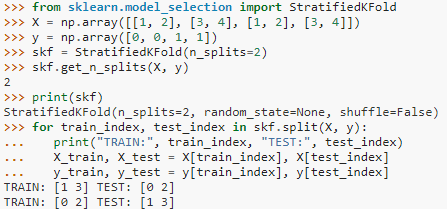
\includegraphics[scale=0.5]{figures/Chapter 7/1164086/Teori/chapter7tasya1.png}
\caption{Ilustrasi KFold Cross Tasya}
\label{Teori}
\end{figure}

\subsubsection{Jelaskan apa maksudnya kode program for train, test in splits.dilengkapi dengan ilustrasi atau gambar.} 
Maksudnya yaitu untuk menguji apakah setiap data pada dataset sudah di split dan tidak terjadi penumpukan. Yang dimana maksudnya di setiap class tidak akan muncul id yang sama. Ilustrasinya misalkan kita memiliki 4 baju dengan model yang berbeda. Kemudian kita bagikan kedua anak, tentunya setiap anak yang menerima baju tidak memiliki baju yang sama modelnya.

\subsubsection{Jelaskan apa maksudnya kode program \emph{train\_content = d['CONTENT'].iloc[train\_idx]} dan \emph{test\_content = d['CONTENT'].iloc[test\_idx]}. dilengkapi dengan ilustrasi atau gambar}

Maksudnya yaitu mengambil data pada kolom atau index CONTENT yang merupakan bagian dari train\_idx dan test\_idx. Ilustrasinya, ketika data telah diubah menjadi train dan test maka kita dapat memilihnya untuk ditampilkan pada kolom yang diinginkan.

\subsubsection{Soal No. 5 Jelaskan apa maksud dari fungsi \emph{tokenizer = Tokenizer(num\_words=2000)} dan \emph{tokenizer.fit\_on\_texts(train\_content)}, dilengkapi dengan ilustrasi atau gambar} 
Dimana variabel tokenizer akan melakukan vektorisasi kata menggunakan fungsi Tokenizer yang dimana jumlah kata yang ingin diubah kedalam bentuk token adalah 2000 kata. Dan untuk \emph{tokenizer.fit\_on\_texts(train\_content)} maksudnya kita akan melakukan fit tokenizer hanya untuk dat trainnya saja tidak dengan data test nya untuk kolom CONTENT. Ilustrasinya, Jadi, jika Anda memberikannya sesuatu seperti, "Kucing itu duduk di atas tikar." Ini akan membuat kamus s.t. word\_index ["the"] = 0; word\_index ["cat"] = 1 itu adalah kata -> kamus indeks sehingga setiap kata mendapat nilai integer yang unik.

\subsubsection{Jelaskan apa maksud dari fungsi \emph{d\_train\_inputs = tokenizer.texts\_to\_matrix(train\_content, mode='tfidf')} dan \emph{d\_test\_inputs = tokenizer.texts\_to\_matrix(test\_content, mode='tfidf')}, dilengkapi dengan ilustrasi kode dan atau gambar} 


Maksudnya yaitu untuk variabel d\_train\_inputs akan melakukan tokenizer dari bentuk teks ke matrix dari data train\_content dengan mode matriksnya yaitu tfidf begitu juga dengan variabel d\_test\_inputs untuk data test. Berikut gambar ilustrasinya
\begin{figure}[ht]
\centering
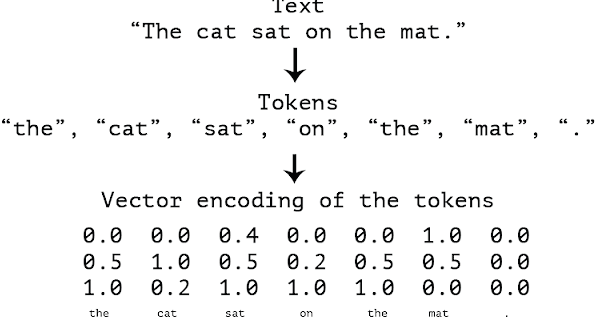
\includegraphics[scale=0.5]{figures/Chapter 7/1164086/Teori/chapter7tasya2.png}
\caption{Ilustrasi Text To Matrix Tasya}
\label{Teori}
\end{figure}

\subsubsection{Jelaskan apa maksud dari fungsi \emph{d\_train\_inputs = d\_train\_inputs/np.amax(np.absolute(d\_train\_inputs))} dan \emph{d\_test\_inputs = d\_test\_inputs/np.amax(np.absolute(d\_test\_inputs))}, dilengkapi dengan ilustrasi atau gambar}

Fungsi tersebut akan membagi matrix tfidf tadi dengan amax yaitu mengembalikan maksimum array atau maksimum sepanjang sumbu. Yang hasilnya akan dimasukan kedalam variabel d\_train\_inputs untuk data train dan d\_test\_inputs untuk data test dengan nominal absolut atau tanpa ada bilangan negatif dan koma.
\begin{figure}[ht]
\centering
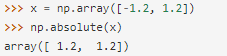
\includegraphics[scale=0.5]{figures/Chapter 7/1164086/Teori/chapter7tasya4.png}
\caption{Ilustrasi np Absolute Tasya}
\label{Teori}
\end{figure}



\subsection{Praktek}


\subsection{Penanganan Error}
